\section{Distanzermittlung von Klauseln in Sha256}
\label{sec:ana:distance}

Die Analyse der neuen Klauseln aus der Kompressionsfunktion erfolgt auf Basis einer Distanzmetrik. Je höher die Distanz einer Klausel, desto höher
ist ihr angenommener Wert. Eine hohe Distanz bedeutet, dass die Klausel Literale aus Modulen in Zusammenhang bringt, die bisher in keiner direkten
Beziehung stehen.

Für die Distanzberechnung wird ein ungerichteter Graph aus den Modulen mit Level 10 erstellt. Ein Modul definiert sich dabei aus zusätzliche Literalen
und den Ausgangsliteralen. Im Gegensatz zum letzten Abschnitt fallen die Eingangsliterale weg, um eine eindeutige Zuordnung eines Literals zu einem
Modul durchführen zu können. Realisiert wird der Graph durch einen Collector mit dem Namen "`ModulGraph"'. Genau wie die ModulDB aus dem letzten Abschnitt
überschreibt der ModulGraph nur die Methode newModul des Collectors, um die Registrierung der Module zu erfassen. Um die Zuordnung der Literale zu einem
Modul schnellstmöglich durchführen zu können, wird eine Lookup-Tabelle erstellt, in der zu jedem Literal das zugehörige Modul hinterlegt ist. Registriert
sich ein Modul im ModulGraph, erfolgt zunächst die Aufnahme in die Lookup-Tabelle. Direkt im Anschluss wird das Modul mit den Modulen verknüpft, die die
Eingangswerte liefern, und so der ungerichtete Graph erstellt.

Der ModulGraph stellt eine Funktion "`printGraph"' bereit, mit der der ungerichtete Graph visualisiert werden kann. Die Ausgabe erfolgt in der Sprache DOT \cite{lang:dot}
mit der Graphen einfach beschrieben werden können. Mit Hilfe eines Renderes kann die Beschreibung des Graphen in ein Grafikformat überführt werden.
Optional kann als Parameter eine Klausel übergeben werden um Module, deren Literale in der Klausel vorkommen, farblich hervorzuheben. Abbildung \ref{fig:sha256_graph}
zeigt einen Ausschnitt aus dem vollständigen Graphen der Kompressionsfunktion. Abgebildet ist die dritte Anwendung der Rundenfunktion. Neben den
Modulnamen werden die verwendeten Literale ausgegeben. Da der Addierer zusätzliche Literale benötigt (Carrybits), sind bei diesem zwei Bereiche aufgeführt.
Die anderen Module kommen ohne zusätzliche Literale aus und enthalten somit nur die Ausgangsliterale. Anzumerken sind die fünf ausgehenden Kanten der beiden
finalen Addierer der Rundenfunktion. Die Ergebnisse werden jeweils in den vier folgenden Runden in fünf weiteren Modulen verwendet.
\begin{figure}[!h]
  \centering
  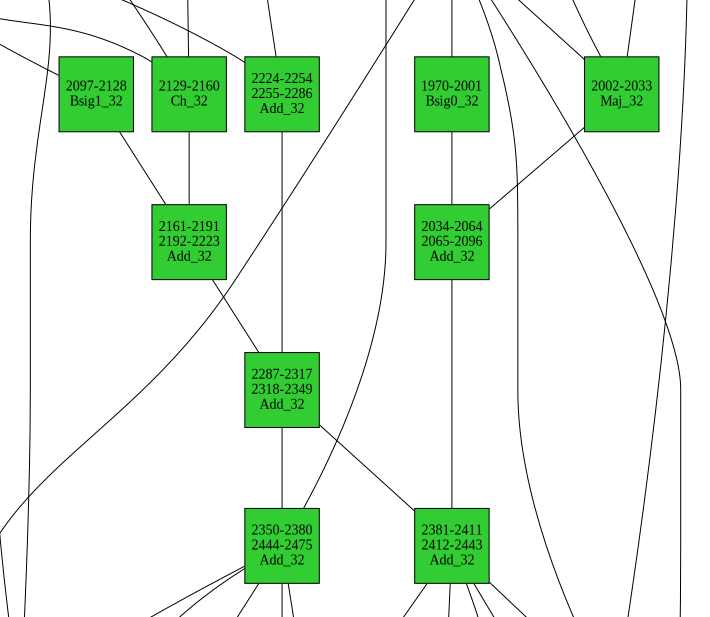
\includegraphics[scale=0.43]{images/sha256graph}
  \caption{Ausschnitt des ungerichteten Graphen von \glos{sha256}}
  \label{fig:sha256_graph}
\end{figure}

Nach der Erstellung des Graphs werden die Distanzen der Module untereinander berechnet. Für jedes Modul wird dafür der Dijkstra-Algorithmus \cite{dijkstra} angewandt,
um die Distanzen zu allen anderen Modulen zu berechnen. Jede Kante bekommt dabei das Gewicht eins. Genau wie für die Zuordnung der Literale zu den Modulen wird für
die Distanzermittlung eine Lookup-Tabelle verwendet. In jedem Knoten werden so die Distanzen zu allen anderen Modulen abgelegt. Für die vollständige Kompressionsfunktion
von \glos{sha256} stellt sich heraus, dass die größte Distanz zwischen zwei Modulen sechzehn beträgt; Es liegen somit maximal fünfzehn Module zwischen zwei anderen
Modulen. Berechnet werden durch den Dijkstra-Algorithmus auch die Wege für die die Distanz gilt. Die Wege haben jedoch für diese Arbeit keine Relevanz und werden
verworfen. Durch die Lookup-Tabellen kann die Berechnung der Distanzen einmalig bei Programmstart erledigt werden und große Klauselmengen können effizient bewertet werden.

Nachdem die Distanzen der einzelnen Module bekannt sind, kann damit die Distanz einer Klausel berechnet werden. Da eine Klausel mehr als zwei Module betreffen kann, werden
die Distanzen aller betroffenen Module überprüft und die größte Distanz ausgewählt. Ermittelt wird außerdem die Anzahl der betroffenen Module. Ein Klausel mit sechs Literalen
kann zum Beispiel zwei Module betreffen, wenn je drei Literale aus einem Modul stammen. Die Distanz einer Klausel ergibt sich aus der Formel in Abbildung \ref{eq:clausedistance}.
\begin{figure}[!h]
  \begin{align*}
  Klauseldistanz = gr\ddot{o}{\beta}te~Moduldistanz - Modulanzahl + 1
  \end{align*}
  \caption{Formel zur Berechnung der Distanz einer Klausel}
  \label{eq:clausedistance}
\end{figure}

Die Formel soll anhand eines Beispiels erläutert werden. 4 Literale, 3 Module, 3 MaxDist, ergeben 1 übersprungenes modul im schlechtesten fall. \TODO{ausführen}

\begin{figure}[!h]
  \centering
  \begin{minipage}[b]{6cm}
    \centering
    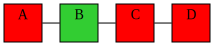
\includegraphics[scale=0.6]{images/distance1}\\
    Schlechtester Fall
  \end{minipage}
  \begin{minipage}[b]{6cm}
    \centering
    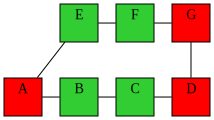
\includegraphics[scale=0.6]{images/distance2}\\
    Möglicher Fall
  \end{minipage}
  \caption{Beispiel für die Distanz einer Klausel}
  \label{fig:distance}
\end{figure}

Das Programm "`distancechecker"'

Ausgabe in eine DIMACS-Datei je distance

\TODO{erledigen}